\documentclass[12pt, final]{article}
\usepackage{color}
\usepackage{times}
\usepackage{amssymb,amsmath,amsthm}
\usepackage{comment}
\usepackage{dsfont}
\usepackage{graphicx}
\usepackage{enumerate}
\usepackage{enumitem}
\usepackage[paperwidth=8.5in,left=1.0in,right=1.0in,top=1.0in,bottom=1.0in,paperheight=11.0in]{geometry}
\usepackage[labelsep=colon,singlelinecheck=false,footnotesize]{caption}
\usepackage{fancyhdr}
\usepackage{float}
\usepackage{booktabs}
\usepackage[sort&compress]{natbib}
\usepackage{subfig}
\usepackage{titlesec}
\usepackage[breaklinks]{hyperref}
\hypersetup{pdfdisplaydoctitle=true,bookmarksnumbered=true,colorlinks=true,citecolor=black,linkcolor=darkblue,urlcolor=darkred,pdfstartview=FitH,pdfpagemode=UseNone}
\usepackage[hyphenbreaks]{breakurl}
\usepackage{accents}
\newcommand{\ubar}[1]{\underaccent{\bar}{#1}}
\usepackage{epstopdf}
\epstopdfsetup{outdir=./}
\usepackage{xcolor}
\usepackage{setspace}
\def\changemargin#1#2{\list{}{\rightmargin#2\leftmargin#1}\item[]}
\let\endchangemargin=\endlist 
\newcommand{\forceindent}{\leavevmode{\parindent=15pt\indent}}


%Define Color Names
\definecolor{Gray}{rgb}{0.65,0.65,0.65}
\definecolor{darkblue}{rgb}{0,0,0.55}
\definecolor{darkred}{rgb}{0.5,0,0}

%Section Headings
\newcommand\Bheadfont{\fontsize{14pt}{\baselineskip}\selectfont}
\titleformat{\section}[hang]{\normalfont\sc\color{darkblue}\Bheadfont}{\thesection\hskip0.618em}{0em}{}
\titlespacing*{\section}{0pt}{15pt plus 2pt minus 2pt}{9pt plus 2pt minus 2pt}
\titleformat{\subsection}[runin]{\normalfont\sc\color{darkblue}} {\thesubsection\hskip0.618em}{0em}{}
\titlespacing*{\subsection}{0pt}{13pt plus 2pt minus 2pt}{13pt plus 2pt minus 2pt}
\titleformat{\subsubsection}[runin]{\normalfont\sc\color{darkblue}} {\thesubsubsection\hskip0.618em}{0em}{}
\titlespacing*{\subsubsection}{0pt}{13pt plus 2pt minus 2pt}{13pt plus 2pt minus 2pt}
\titleformat{\paragraph}[runin]{\bfseries}{\theparagraph\hskip0.618em}{0em}{}
\titlespacing*{\paragraph}{0pt}{13pt plus 2pt minus 2pt}{13pt plus 2pt minus 2pt}

\title{Comparison of Global Solution Methods to a Zero Lower Bound Model}
\date{\small\today}
\author{Emily Martell\thanks{Thank you to Professor Throckmorton for advising and providing materials for this project. Thank you to Professor Campbell, Professor Han, Professor Rolek, and Professor Throckmorton for serving on my committee.}}
\begin{document}
\maketitle
\bigskip
\begin{center}
\fontsize{14pt}{\baselineskip}\sc Abstract%\normalfont
\end{center}

\onehalfspacing
\begin{changemargin}{1cm}{1cm}

{\small \forceindent During the Great Recession, the U.S. Federal Reserve lowered policy rates to zero, introducing a kink in its policy rule and calling into question traditional solution methods. Recent papers have solved fully nonlinear models that treats the zero lower bound (ZLB) as an occasionally binding constraint, but there is little work analyzing the relative performance of these nonlinear solution methods. Two proposed solution methods are policy function iteration with linear interpolation and regime-indexed policy function iteration with Chebyshev polynomial approximation. We examine the impact of making the policy functions conditional on whether the ZLB binds. Our solution algorithm uses evenly-spaced grid points, linear interpolation, and Rouwenhorst integration. This paper shows that the regime-indexed policy functions are quite nonlinear in a New Keynesian model with capital and are costly to approximate in terms of solution time.}


\end{changemargin}
\vfill
\pagebreak

\section{Introduction}

As a result of the global financial crisis of 2007-9 and the subsequent recession, central banks lowered
their policy rate to its zero lower bound (ZLB). Although the ZLB constraint has always existed,
for most of the data prior to the recession, policy rates were well above zero. In the wake of this
unprecedented lowering of policy rates, the ZLB holds for a considerable portion of historic data
for three major economies --- the US, Japan, and the Euro Area. The ZLB introduces a kink in the policy
rule and calls into question linear estimation methods. 

Researchers have responded to this inherent
nonlinearity in different ways. Some have failed to incorporate the ZLB period data. Others have
chosen to estimate linear models on the entire data set; however, this could lead to inaccurate estimates
of model parameters and model predictions. Some have estimated a piecewise linear version of the nonlinear model (e.g., \hyperlink{Guerrieri}{\color{black}{Guerrieri and Iacoviello, 2017}}). A few have estimated fully nonlinear models that treats the
	ZLB as an occasionally binding constraint (e.g., \hyperlink{Gust}{\color{black}{Gust et al.,\ 2017}}; \hyperlink{Plante}{\color{black}{Plante et al.,\ 2018}}; \hyperlink{RT}{\color{black}{Richter and Throckmorton, 2016}}). These papers solve the nonlinear model using projection methods, which is explored in several other papers (e.g. \hyperlink{Aruoba}{\color{black}{Aruoba et al.,\ 2018}}; \hyperlink{Fernandez}{\color{black}{Ferna\'ndez-Villaverde et al.,\ 2015)}}. Solving a nonlinear model using projection methods provides the most comprehensive treatment of the ZLB but is computationally intensive.

As it is important to incorporate all historical data and yield accurate parameter values and predictions, the path forward seems to be in fully nonlinear models. Among those that use projection methods to solve a nonlinear model, some use policy function iteration with linear interpolation (e.g., \hyperlink{Plante}{\color{black}{Plante et al.,\ 2018}}; \hyperlink{RT}{\color{black}{Richter and Throckmorton, 2016}}). In terms of the approximating function, others estimate alternative functions like regime-indexed policy functions (\hyperlink{Gust}{\color{black}{Gust et al.,\ 2017}}) or piecewise smooth policy functions (\hyperlink{Aruoba}{\color{black}{Aruoba et al.\ 2018}}) to avoid the kink introduced by the ZLB.  With respect to the grid construction, some use the Smolyak collocation method developed by \hyperlink{Judd}{\color{black}{Judd et al.\ (2010)}} to reduce the burden of dimensionality (e.g., \hyperlink{Gust}{\color{black}{Gust et al.,\ 2017}}; \hyperlink{Fernandez}{\color{black}{Ferna\'ndez-Villaverde et al.\, 2015}}; \hyperlink{Aruoba}{\color{black}{Aruoba et al.,\ 2018}}).
Not much work has been done in comparing the accuracy and speed of different global nonlinear solution methods. We will  examine the performance of \hyperlink{Atkinson}{\color{black}{Atkinson et al.\ (2019)}} and \hyperlink{Gust}{\color{black}{Gust et al.\ (2017)}} in terms of accuracy and speed as examples of different ways to solve nonlinear models. 

The \hyperlink{Atkinson}{\color{black}{Atkinson et al.\ (2019)}} solution method is policy function iteration with linear interpolation to approximate future variables.  The state space features evenly-spaced nodes and exogenous state variables  approximated with the Markov chain from \hyperlink{Rouwenhorst}{\color{black}{Rouwenhorst (1995)}}, which \hyperlink{Kopecky}{\color{black}{Kopecky and Suen (2010)}} show outperforms other methods for approximating autoregressive processes. The Rouwenhorst approximation is useful because it only requires interpolation along the dimensions of the endogenous state variables. They update the policy functions with linear interpolation to accurately capture the kink experienced at the ZLB.

The \hyperlink{Gust}{\color{black}{Gust et al.\ (2017)}} solution method approximates policy functions underlying the model's decision rule using an antistropic Smolyak method with Chebyshev polynomials. (See \hyperlink{Judd2}{\color{black}{Judd et al.\, 2014}} for a discussion of antistropic Smolyak methods). They approximate the exogenous state variables using Gauss-Hermite quadrature. Instead of directly computing the policy functions, they estimate functions at and away from the ZLB, which builds on \hyperlink{Christiano}{\color{black}{Christiano and Fisher (2000)}}. The idea is that the policy functions feature a kink or non-differentiability at the ZLB and regime-indexing the policy functions will yield smoother functions. This is appropriate for the choice of Chebyshev polynomial approximation, which performs better on smoother functions. 

In this paper, we consider the effect of making the policy functions conditional on whether the ZLB binds. To isolate the effect of splitting the policy functions, we use policy function iteration on a fixed point with linear interpolation following \hyperlink{Atkinson}{\color{black}{Atkinson et al.\ (2019)}}. This solution method directly computes the policy functions, while the \hyperlink{Gust}{\color{black}{Gust et al.\ (2017)}} solution method indirectly computes the policy functions through regime-indexed policy functions. Henceforth, the solution method based on the \hyperlink{Atkinson}{\color{black}{Atkinson et al.\ (2019)}} solution algorithm will be denoted ART and the solution algorithm that estimates smoother functions based on \hyperlink{Gust}{\color{black}{Gust et al.\ (2017)}} will be denoted GHLS. It is important to note that we do not consider the effect of a Smolyak basis with Chebyshev polynomials, so this is a modified \hyperlink{Gust}{\color{black}{Gust et al.\ (2017)}} solution method. The key point in this paper is to explore how splitting up the policy functions conditional on the ZLB impacts the speed and accuracy of the solution of a nonlinear model. 

First, we construct the state space with evenly-spaced nodes and approximate the exogenous state variables with \hyperlink{Rouwenhorst}{\color{black}{Rouwenhorst (1995)}}. After obtaining initial conjectures for a set of policy functions from the log-linear solution, we iterate on the policy functions, linearly interpolating and numerically integrating the policy functions each step, using a fixed point iteration scheme. The algorithm converges once the maximum distance between successive guesses of policy functions falls below a convergence criterion. For the ART portion, we update a single policy function. For the GHLS portion, we update regime-indexed policy functions.

%In a NK model instead???
The interest rate enters directly in the consumption Euler equation, which for our small-scale model without habit formation is as follows:
\begin{gather*}
    1 = \beta E_t[(c_t/c_{t+1})(s_ti_t/\pi_{t})],
\end{gather*}
where $E_t$ is the expectation operator, $0<\beta<1$ is the discount factor, and $c_t$, $s_t$, $i_t$, and $\pi_t$ are consumption, the risk premium, the interest rate, and inflation at time $t$. The interest rate appears because the household has the choice of owning a nominal bond, and must choose a combination of consumption, labor, and bond holdings to maximize expected lifetime utility. For this reason, consumption $c_t$ depends on the interest rate. At the ZLB, the presence of the interest rate creates a nonlinearity in the consumption Euler equation and motivates the use of regime-indexed policy functions. 

To approximate regime-indexed consumption policy functions $c_t^{ZLB}$ and $c_t^{normal}$, we provide initial guesses based on the log-linear solution. We refine the policy function guesses as follows: For each node in the state space, we solve for the time $t$ variables with either $c_t^{ZLB}$  or $c_t^{normal}$ according to $i_t$, the interest rate at time $t$. With the time $t$ variables, we linearly interpolate both policy functions. Next, we calculate the interest rate on each node in the state space, construct an aggregate consumption policy function based on whether the economy is at the ZLB on each node, and calculate time $t+1$ variables accordingly. We then update $c_t^{ZLB}$ with the interest rate constrained at the ZLB, and $c_t^{normal}$ with a positive interest rate.

%It might help to explain in the intro the key difference in the approximation of the policy functions. You could show a standard Euler Equation, point out the nominal interest rate, and then explain you would approximate a policy function for consumption that depends on whether the economy is at the ZLB. 

In terms of accuracy, both ART and GHLS yield similar Euler equation errors, with ART being slightly more accurate for the model with capital. The ART method converges much more quickly than the GHLS method, particularly when capital is introduced to the model. There is not a clear advantage of the regime-indexed policy function approximation when using an evenly spaced grid with linear interpolation. All else equal, using regime-indexed policy functions increases the computing time. However, introducing Chebyshev polynomials and sparse grid methods as in \hyperlink{Gust}{\color{black}{Gust et al.\ (2017)}} may reduce solution time and allow us to solve larger models with more state variables. Further research could explore how much accuracy is gained or lost relative to using non regime-indexed policy functions approximated with Chebyshev polynomials. 

The remainder of the paper is as follows: \hyperlink{Section 2}{Section 2} outlines our setup for the model with capital. \hyperlink{Section 3}{Section 3} describes regime-indexed polynomials and outlines the solution algorithm. \hyperlink{Section 4}{Section 4} discusses the results in terms of solution time, curvature of policy functions, and Euler equation errors. \hyperlink{Section 5}{Section 5} concludes.

\section[Section 2]{Model \hypertarget{Section 2}{}} 
Our model is a widely-employed New Keynesian model which is similar to the model in \hyperlink{Atkinson}{\color{black}{Atkinson et al.\ (2019)}}, but includes capital accumulation as in \hyperlink{Gust}{\color{black}{Gust et al.\ (2017)}}. Thus, it is an appropriate model to benchmark the accuracy and speed of the two solution methods.

\subsection{Firms} The production sector consists of a continuum of monopolistically competitive intermediate goods firms and a final goods firm. Intermediate firm $f \in [0,1]$ produces a differentiated good, $y(f)$, according to $y_t(f) = (k_{t-1}(f))^\alpha(z_tn_t(f))^{1-\alpha}$, where $n(f)$ is the labor hired by firm $f$ and $k(f)$ is the capital rented by firm $f$. $z_t = g_tz_{t-1}$ is technology, which is common across firms. Deviations from the steady-state growth rate, $\bar{g}$, follow
\begin{gather}
  \label{eq:1}
  g_t = \bar{g} + \sigma_g\varepsilon_{g,t},\; \varepsilon_g \sim \mathds{N}(0,1). 
\end{gather}

The final goods firm purchases output from each intermediate firm to produce the final good, $y_t \equiv [\int_{0}^1 y_t(f)^{(\theta-1)/\theta}df]^{\theta/(\theta-1)}$, where $\theta > 1$ is the elasticity of substitution. Dividend maximization determines the demand for intermediate good $f$, $y_t(f) = (p_t(f)/p_t)^{-\theta}y_t$, where $p_t = [\int_{0}^{1} p_t(f)^{1-\theta}df]^{1/(1-\theta)}$ is the price level. Following \hyperlink{Rotemberg}{\color{black}{Rotemberg (1982)}}, intermediate firms pay a price adjustment cost, $adj_t^p(f) \equiv \varphi(p_t(f)/(\bar{\pi}p_{t-1}(f))-1)^2)y_t/2$, where $\varphi > 0$ scales the cost and $\bar{\pi}$ is the steady-state gross inflation rate. Given this cost, firm $f$ chooses $n_t(f)$, $k_{t-1}(f)$, and $p_t(f)$ to maximize the expected discounted present value of future dividends, $E_t\sum_{k=t}^\infty q_{t,k}d_k(f)$, subject to its production function and the demand for its product, where $q_{t,t} \equiv 1$, $q_{t,t+1} \equiv \beta(\lambda_t/\lambda_{t+1})$ is the pricing kernel between periods $t$ and $t+1$, $q_{t,k} \equiv \prod_{j=t+1}^{k>t} q_{j-1,j}$, and $d_t(f) = p_t(f)y_t(f)/p_t - w_tn_t(f) - adj_t^p(f)$. In symmetric equilibrium, the optimality conditions reduce to
\begin{gather}
  y_t = (k_{t-1})^\alpha(z_tn_t)^{1-\alpha},\\
  w_t = (1-\alpha)mc_ty_t/n_t,\\
  r_t^k = \alpha mc_t y_t/k_{t-1},\\
  \varphi(\pi_t^{gap}-1)\pi_t^{gap} = 1-\theta + \theta mc_t + \beta\varphi E_t[(\lambda_t/\lambda_{t+1})(\pi_{t+1}^{gap}-1)\pi_{t+1}^{gap}(y_{t+1}/y_t)],
\end{gather}
where $\pi^{gap}_t = \pi_t/\bar{\pi}_t$ and $\pi_t = p_t/p_{t-1}$ is the gross inflation rate. If $\varphi = 0$, the real marginal cost of producing a unit of output ($mc_t$) equals $(\theta-1)/\theta$, which is the inverse of the markup of price over marginal cost.
\subsection{Households} The households choose $\{c_t, n_t, b_t, x_t, k_t\}_{t=0}^\infty$ to maximize expected lifetime utility given by $E_0\sum_{t=0}^\infty\beta[\log(c_t-hc^a_{t-1}) - \chi n_t^{1+\eta}/(1+\eta)]$, where $\beta$ is the discount factor, $\chi > 0$ determines steady-state labor, $1/\eta$ is the Frisch elasticity of labor supply, $c$ is consumption, $c^a$ is aggregate consumption, $h$ is the degree of external habit persistence, $b$ is the real value of a privately-issued 1-period nominal bond, $x$ is investment, and $E_0$ is an expectation operator conditional on information available in period 0. The household's budget constraint is given by
\begin{gather*}
    c_t+x_t+b_t/(i_ts_t)=w_tn_t+r_t^kk_{t-1}+b_{t-1}/\pi_t+d_t,
  \end{gather*}
where $i$ is the gross nominal interest rate, $r^k$ is the capital rental rate, and $d$ is a real dividend from ownership of intermediate firms. The nominal bond, $b$ is subject to a risk premium, $s$, that follows
\begin{gather}
  \label{eq:6}
  s_t = (1-\rho_s)\bar{s} + \rho_ss_{t-1} + \sigma_s\varepsilon_{s,t},\; 0 \leq \rho_s < 1,\; \varepsilon_s \sim \mathds{N}(0,1),
\end{gather}
where $\bar{s}$ is the steady-state value. An increase in $s_t$ boosts saving, which lowers period-$t$ demand.

Households also face an investment adjustment cost, so the law of motion for capital is given by
\begin{gather}
  k_t = (1-\delta)k_{t-1} + x_t(1-\nu(x^g_t - 1)^2/2),\; 0 \leq \delta \leq 1,
  \end{gather}
where $x_t^g = x_t/(\bar{g}x_{t-1})$ is investment growth relative to its steady-state and $\nu \geq 0$ scales the cost.

The first order conditions to each household's constrained optimization problem are given by
\begin{gather}
  \lambda_t = c_t - hc^a_{t-1}, \\
  w_t = \chi n_t^\eta \lambda_t,\\
  1 =  \beta E_t[(\lambda_t/\lambda_{t+1})(s_ti_t/(\bar{\pi}\pi_{t+1}^{gap}))],\\
  q_t = \beta E_t[(\lambda_t/\lambda_{t+1})(r^k_{t+1}+(1-\delta)q_{t+1})],\\
  1 = q_t[1-\nu(x^g_t-1)^2/2 - \nu(x_t^g-1)x_t^g] + \nu\beta\bar{g}E_t[q_{t+1}(\lambda_t/\lambda_{t+1})(x^g_{t+1})^2(x^g_{t+1}-1)],\\
  \varphi(\pi_t^{gap}-1)\pi_t^{gap} = 1-\theta + \theta mc_t + \beta\varphi E_t[(\lambda_t/\lambda_{t+1})(\pi_{t+1}^{gap}-1)\pi_{t+1}^{gap}(y_{t+1}/y_t)],
\end{gather}
where $1/\lambda$ is the marginal utility of consumption and $q$ is Tobin's q.\\

\noindent
\textbf{Monetary Policy} The central bank sets the gross nominal interest rate, $i$, according to
\begin{gather}
    \label{eq:15}
    i_t=\max\{1,i_t^n\},\\
      \label{eq:16}
  i_t^n=(i^n_{t-1})^{\rho_i}(\bar{\imath}(\pi^{gap}_t)^{\phi_\pi}(y^{gdp}_{t})^{\phi_y})^{1-\rho_i}\exp(\sigma_i\varepsilon_{i,t}), 0 \leq \rho_i < 1, \varepsilon_i \sim \mathds{N}(0,1),
  \end{gather}
where $y^{gdp}$ is real GDP (i.e., output, $y$, minus the resources lost due to adjustment costs, $adj^p$), $i^n$ is the gross notional interest rate, $\bar i$ is the target values of the nominal interest rate, and $\phi_\pi$ and $\phi_y$ are the responses to the inflation and output growth gaps. A more negative net notional rate indicates that the central bank is more constrained.\\

\noindent
\textbf{Competitive Equilibrium} The aggregate resource constraint and real GDP definition are given by
\begin{gather}
  c_t + x_t = y_t^{gdp}\\
  y_t^{gdp} = [1 - \varphi(\pi_t^{gap}-1)^2/2]y_t
\end{gather}
The model does not have a steady-state due to the unit root in technology, $z_t$. Therefore, we define the variables with a trend in terms of technology (i.e., $\tilde{x}_t \equiv x_t/z_t$). The detrended equilibrium system is provided in \hyperlink{Appendix A}{Appendix A}. A competitive equilibrium consists of sequences of quantities, $\{\tilde{c}_t, \tilde{y}_t, \tilde{y}_t^{gdp}, x^g_t, y^g_t, n_t, \tilde{k}_t, \tilde{x}_t\}_{t=0}^\infty$, prices, $\{\tilde{w}_t, i_t, i^n_t, \pi_t, \tilde{\lambda}_t, q_t, r^k_t, mc_t\}_{t=0}^\infty$, and exogenous variables, $\{s_t,g_t\}_{t=0}^\infty$, that satisfy the detrended equilibrium system, given the initial conditions, $\{\tilde{c}_{-1}, i^n_{-1}, \tilde{k}_{-1}, \tilde{x}_{-1}, \tilde{w}_{-1}, s_0, g_0, \varepsilon_{i,0}\}$, and three sequences of shocks, $\{\varepsilon_{g,t}, \varepsilon_{s,t}, \varepsilon_{i,t}\}_{t=1}^\infty$.

\begin{table}[H]
  \hypertarget{Table 1}
\centering
\captionsetup{justification=centering}
  \small
    \setlength{\tabcolsep}{7.5pt}      
  \begin{tabular}{l c c l c c}
    \hline
  Subjective Discount Factor & $\beta$ & $0.9949$ & Rotemberg Price Adjustment Cost & $\varphi$ & $100$ \\
   Frisch Labor Supply Elasticity & $1/\eta$ & $3$ & Inflation Gap Response & $\phi_\pi$ & $2.0$ \\
  Price Elasticity of Substitution & $\theta$ & $6$ & Output Growth Gap Response & $\phi_y$ & $0.5$ \\
  Steady-State Labor Hours & $\bar{n}$ & $1/3$ & Habit Persistence & $h$ & $0.80$ \\
  Steady-State Risk Premium & $\bar{s}$ & $1.0058$ & Risk Premium Persistence & $\rho_s$ & $0.80$ \\
  Steady-State Growth Rate & $\bar{g}$ & $1.0034$ & Notional Rate Persistence & $\rho_i$ & $0.80$ \\
  Steady-State Inflation Rate & $\bar{\pi}$ & $1.0053$ & Technology Growth Shock SD & $\sigma_g$ & $0.005$ \\
  Capital Share of Income & $\alpha$ & $0.35$ & Risk Premium Shock SD & $\sigma_s$ & $0.0085$ \\
  Capital Depreciation Rate & $\delta$ & $0.025$ & Notional Interest Rate Shock SD & $\sigma_i$ & $0.002$ \\
  Investment Adjustment Cost & $\nu$ & $4$ & & &\\
  \hline
  \end{tabular}
  \caption{Parameter values}
  \label{Tab:1}
\end{table}


\subsection{Parameter Values} \hyperlink{Table 1}{Table 1} shows the model parameters. Parameters are from \hyperlink{Atkinson}{\color{black}{Atkinson et al.\ (2019)}}, and are chosen to be characteristic of U.S. data. The subjective discount factor, $\beta$ is set to $0.9949$, the time average of the values implied by the steady-state consumption Euler equation and the federal funds rate. The Frisch labor supply elasticity $1/\eta$ is set to 3 to match the macro estimate in \hyperlink{Peterman}{\color{black}{Peterman (2016)}}. The price elasticity of substitution $\theta$ is set to 6, matching GHLS and corresponding to to a 20\% average markup. Steady-state labor hours $\bar{n}$ is set to 1/3 of available time. The steady-state risk premium, growth rate, and inflation rate are set to the time averages of per capital real DGP growth, the percent GDP implicit price deflator, and the Baa corporate bond yield relative to the yield on the 10-Year Treasury. The capital share of income $\alpha$ is equal to the \hyperlink{Fernald}{\color{black}{Fernald (2012)}} utilization-adjusted quarterly-TFP estimates of the capital share of income from 1988-2017Q4. The other parameters are set to values consistent with posterior estimates from similar models in the literature. For the model without capital, all parameters are equivalent to those above except we set $\sigma_s=0.006$ to allow the GHLS algorithm to converge.

\section[Section 3]{Solution Methods \hypertarget{Section 3}{}} 
\subsection{Regime-indexed policy functions} Instead of directly approximating the policy functions, some papers elect to approximate alternative functions to avoid the kink experienced at the ZLB (e.g., \hyperlink{Gust}{\color{black}{Gust et al.,\ 2017}}; \hyperlink{Aruoba}{\color{black}{Aruoba et al.,\ 2018}}). \hyperlink{Gust}{\color{black}{Gust et al.\ (2017)}} uses policy functions that are indexed by the interest-rate regime. Because these functions do not depend on the current indicator function, \hyperlink{Gust}{\color{black}{Gust et al.\ (2017)}} claims that they are more likely to be smooth. The regime-specific functions still depend on a secondary effect that the non-differentiability in the nominal rate in the following period has on expectations of future variables.  However, following \hyperlink{Christiano}{\color{black}{Christiano and Fisher (2000)}} this effect should be small due to the presence of the expectations operators which act to smooth out regime-specific functions. Let the vector of policy functions at time $t$ be denoted $\textbf{pf}_t$ and the realization on node $d$ be denoted $\textbf{pf}_t(d)$. The idea for regime-indexed policy functions is as follows:
\begin{gather}
    \label{eq:18}
  \textbf{pf}_t(d) = \textbf{pf}_{t,1}(d)\mathds{I}_t(d) + \textbf{pf}_{t,2}(d)(1-\mathds{I}_t(d)),
\end{gather}

where $\mathds{I}_t(d)$ is defined by
\begin{gather}
    \label{eq:19}
  \mathds{I}_t(d) = 
\begin{cases}
     1 &\text{ if } i_t > 1\\
     0 &\text{ otherwise.}
\end{cases}
\end{gather}
The variable $i_t=\max\{1,i_t^n\}$ represents the value of the notional rate derived from evaluating the functions $\textbf{pf}_{t,j}(d)$ for $j \in \{1,2\}$ and using equation (\ref{eq:16}). (For each variable, $j=1$ denotes the function associated with the regime with a positive nominal rate and $j=2$ denotes the function associated with the ZLB regime.) %In calculating the fixed point, we use $i=1$ when the model is in the ZLB regime. 
The functions $\textbf{pf}_{t,j}$ satisfy the residual functions $R_{t,l,j}$ for $l \in \{1,2,3,4\}$ which correspond to the household FOC bond, FOC capital, FOC investment, and the price Phillips curve, respectively, and $j \in \{1,2\}$.
\begin{gather}
\label{eq:20}
  R_{t,1,1} = 1 - s_ti_t\beta E_t[(\lambda_t/\lambda_{t+1})(1/(\bar{\pi}\pi_{t+1}^{gap}))],\\
\label{eq:21}
  R_{t,1,2} = 1 - s_t\beta E_t[(\lambda_t/\lambda_{t+1})(1/(\bar{\pi}\pi_{t+1}^{gap}))],\\
\label{eq:22}
R_{t,2,j} = q_t - \beta E_t[(\lambda_t/\lambda_{t+1})(r^k_{t+1}+(1-\delta)q_{t+1})],\\
 \label{eq:23} 
  \begin{split}
    R_{t,3,j} &= 1 - q_t[1-\nu(x^g_t-1)^2/2 - \nu(x_t^g-1)x_t^g] \\&- \nu\beta\bar{g}E_t[q_{t+1}(\lambda_t/\lambda_{t+1})(x^g_{t+1})^2(x^g_{t+1}-1)], 
  \end{split}
  \\
   \label{eq:24}
  \begin{split}
    R_{t,4,j} &= \varphi(\pi_t^{gap}-1)\pi_t^{gap} - (1-\theta) - \theta mc_t \\&- \beta\varphi E_t[(\lambda_t/\lambda_{t+1})(\pi_{t+1}^{gap}-1)\pi_{t+1}^{gap}(y_{t+1}/y_t)].
    \end{split}
  \end{gather}

\subsection{Solution Algorithm}
Our solution algorithm is as follows: Construct an evenly-spaced grid by discretizing the endogenous state variables and using \hyperlink{Rouwenhorst}{\color{black}{Rouwenhorst (1995)}} method to approximate the exogenous processes for $s_t$, $g_t$, and $\varepsilon_{i,t}$. We use the Rouwenhorst method so that we do not have to interpolate along the dimensions of the exogenous state variables, which is faster and more accurate than quadrature methods.  As above, the vector of policy functions is denoted $\textbf{pf}_t$ and the realization on node $d$ is denoted $\textbf{pf}_t(d)$. Denote the vector of states $\textbf{z}_t$. 
\begin{enumerate} 
\item To construct the initial policy functions $\textbf{pf}_0$, we solve the log-linear analog of our model with the ZLB not imposed using \hyperlink{Sims}{\color{black}{Sims's (2002) \texttt{gensys}}} algorithm. (For GHLS, we initialize the regime-indexed policy functions by setting them to the log-linear solution.)
\item For each node in the state space $d \in \{1,\dots,D\}:$
\begin{enumerate}
\item Solve for the variables dated at time $t$ given $\textbf{pf}_t$ and $\textbf{z}_t$. (For GHLS, we calculate time $t$ variables with the non-ZLB policy functions if the interest rate $i_t > 1$, and the ZLB policy functions if the interest rate $i_t \leq 1$). 
\item  Linearly interpolate the policy functions at the updated state variables $\textbf{z}_{t+1}$ to obtain $\textbf{pf}_{t+1}(m)$ on every integration node $m \in \{1,\dots,M\}$. (For GHLS, we interpolate the non-ZLB and ZLB policy functions separately.)
\item Given the interpolated policy functions $\{\textbf{pf}(m)\}_{m=1}^M$, and integration nodes and weights provided by the Rouwenhorst method, approximate the expectation operators for the model. (For GHLS, use the interest rate array calculated from the interpolated policy functions to determine whether the model is at the ZLB at each node. We construct the aggregate policy functions accordingly, as in (\ref{eq:18}) and (\ref{eq:19}).)
\item Solve for time $t+1$ variables from the expectation operators. Back out the policy functions $\textbf{pf}_t(d)$ from the expectation operators and time $t+1$ variables. (For GHLS, we solve for the regime-indexed policy functions according to (\ref{eq:20})-(\ref{eq:24})).
\end{enumerate}
\item Repeat step 2 until the maximum distance between successive approximations of the policy functions is below $10^{-6}$. 
\end{enumerate}

  \subsection{Euler Equation Errors}
We use Euler equation errors to measure the accuracy of our solutions. To approximate errors between nodes, we use Gauss-Hermite quadrature instead of the Rouwenhorst method following ART to allow exogenous variables to have realizations between grid points. The Euler equation errors are represented in absolute value of the errors in base 10 logarithms. An Euler equation error of -3 means the household makes an error equivalent to one per 1,000 consumption goods; i.e., an error of 0.1\% on average.

We simulate 10,000 periods of the model using the nonlinear solution with random shocks. For
each period, we follow one iteration of step 2 of the algorithm outlined in Appendix B and then
transform the residuals to Euler equation errors.

	We considered adding a second measure of accuracy, a statistical measure from \hyperlink{Den}{\color{black}{Den Haan and Marcet (1994)}} based on a transformation of the Euler equation residuals to a chi-square distribution. However, it proved uninformative, as several runs of the test statistic were all in the extreme
tails of the distribution.

\section[Section 4]{Results \hypertarget{Section 4}{}} 

\begin{table}[H]
  \centering
\captionsetup{justification=centering}
  \hypertarget{Table 2}
  \small
    \setlength{\tabcolsep}{6pt}      
  \begin{tabular}{l c c c c c c}
    \hline
    & \multicolumn{3}{c}{Model without capital} & \multicolumn{3}{c}{Model with capital} \\
    & Total nodes & Iterations & Total Time & Total Nodes & Iterations & Total time\\
    \hline
  ART & 2401  & 76 & 23.01s (avg. 30 runs) & 78125 & 56 & 0h 9m 16.1s\\    
  GHLS & 2401  & 62 & 19.34s (avg. 30 runs) & 78125 & 1231 &  3h 28m 28.8s\\
  \hline
\end{tabular}
  \caption{Solution times}
\end{table}

\subsection{Solution Times}
\hyperlink{Table 2}{Table 2} reports the solution times for the ART and
GHLS solution methods for the models with and without capital. The solution times
were computed with multi-core processing using the Parallel Computing Toolbox. With MATLAB
executable functions (MEX) provided by the companion toolbox to \hyperlink{RTW}{\color{black}{Richter et al. (2014)}}, we implemented the interpolation steps of the algorithm in Fortran. The solution times represent one run
of each algorithm. The machine used to compute the solutions has 32 total cores (two CPUs at 2.30GHz, each
with 16 cores).

The GHLS method is slightly faster for the model without capital, but much slower for the model with capital. The performance is somewhat contingent upon the
parameterization, but the results indicate that the speed differential blows up for the model with capital. This may be due to the following: The GHLS solution
algorithm has a labor policy (consumption policy for model without capital) both at and away from
the ZLB. As a result, the solution algorithm requires an additional interpolation step. In addition, the GHLS solution algorithm must determine at which nodes the state space is at the ZLB, and
solve for time $t$ and $t + 1$ variables accordingly.

\begin{figure}[H]
\hypertarget{Figure 1}  
    \centering
\captionsetup{justification=centering}
    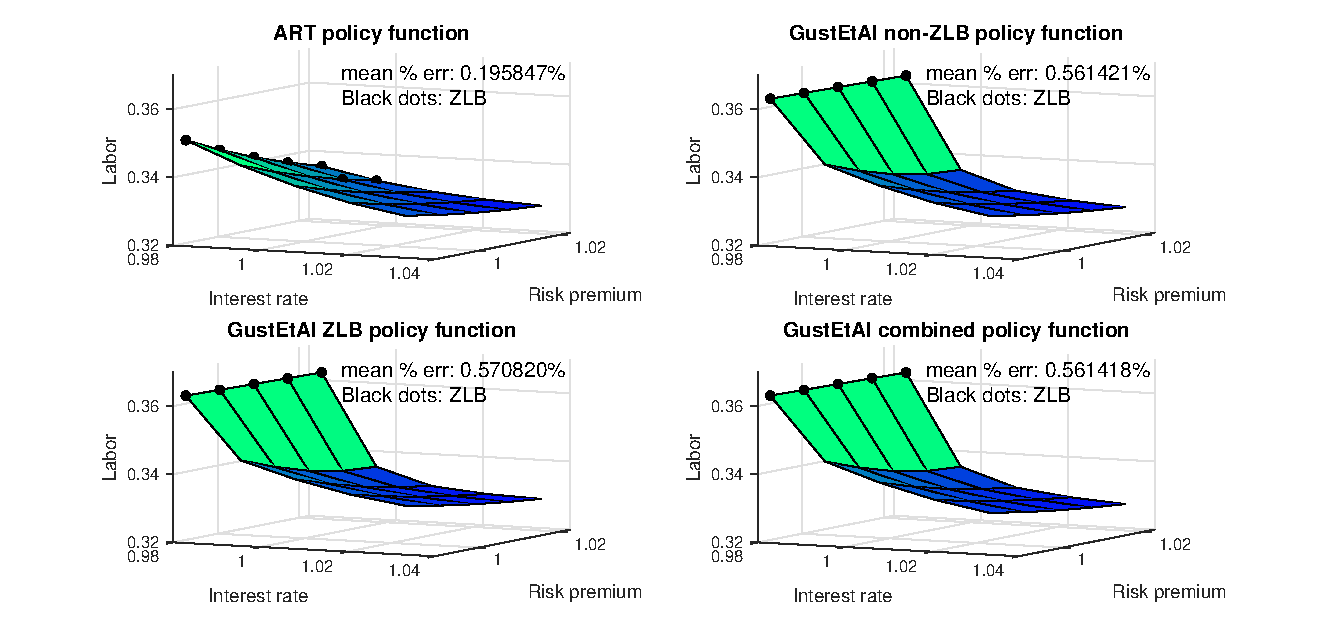
\includegraphics[width=17.25cm,scale=1]{pfs3DCAP.pdf}
  \caption{Labor policy function for model with capital}    
  \label{Fig:1}
  \end{figure}

\subsection{Policy Functions} \hyperlink{Figure 1}{Figure 1} shows the cross-section of the labor policy functions with the interest rate and risk premium for the model with capital. The black dots on the nodes of the
graph represent labor values corresponding to the ZLB. The GHLS labor policy function is
computed at and away from the ZLB and combined later, and all three are shown in the figure. The
GHLS combined policy function is very similar to the policy function away from the ZLB, as only a fraction of the nodes experience the ZLB binding.

Visually, the ART labor policy function cross-section is quite a bit smoother. Labor hours smoothly
increase as the interest rate falls and hits the ZLB. The GHLS labor policy function
features a kink at the ZLB where labor rises dramatically.


\begin{figure}[H]
\hypertarget{Figure 2}  
    \centering
\captionsetup{justification=centering}
    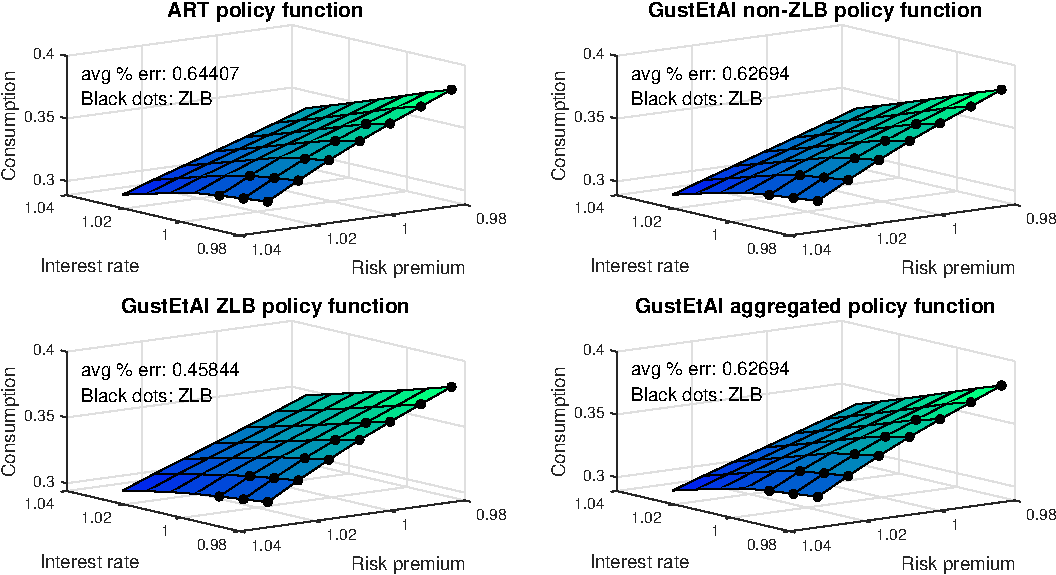
\includegraphics[width=16cm,scale=.9]{pfs3D.pdf}
  \caption{Consumption policy function for model without capital}    
  \end{figure}

\hyperlink{Figure 2}{Figure 2} shows the cross-section of the consumption policy functions with the interest rate and
risk premium. The policy functions are all fairly smooth and only have a slight nonlinearity at the
ZLB. The GHLS policy functions do not experience a profound nonlinearity as they do in the model with capital. The GHLS policy functions are smoother than the ART policy function with respect to both the average percent error from a linear plane and the RMSE.

\begin{table}[H]
  \centering
\captionsetup{justification=centering}
  \hypertarget{Table 3}
  \small
    \setlength{\tabcolsep}{10pt}      
  \begin{tabular}{l c c c c}
    \hline
    & \multicolumn{2}{c}{Model without capital} & \multicolumn{2}{c}{Model with capital} \\
    & Mean \% Error & RMSE & Mean \% Error & RMSE\\
    \hline
    ART policy & 0.64407\% &0.0027327 $c$  units & 0.271154\% & 0.0039806 $l$ units \\    
  GHLS policy & 0.62694\% & 0.0026704 $c$ units & 0.578098\% & 0.0080785 $l$ units \\
  \hline
\end{tabular}
  \caption{Smoothness measures for labor policy functions ($c$ for model with capital and $n$ for model with capital). GHLS combined policy functions are reported.}
\end{table}  

 \hyperlink{Table 3}{Table 3} reports the RMSE (root mean square error) and mean percent error from linear policy
functions. The mean percent error is calculated as $1/M\sum_{i=1}^N[\tilde{\textbf{n}}(i)-\hat{\textbf{n}}(i)]/\bar{n}$
where $N$ is the
number of periods, $\tilde{\textbf{n}}$ is the nonlinear approximation of the labor policy function, $\hat{\textbf{n}}$ is the linear regression model of $\tilde{\textbf{n}}$ fit to
the state variables, and $\bar{n}$ is steady state labor. The linear regression model $Y = XB$ is as follows:
\small
\begin{gather*}
  Y = \tilde{\textbf{n}},
  X = \begin{bmatrix}
    1 & g_t \\ 
    1 & s_t \\   
    1 & mp_t \\
    1 & in_t \\
    1 & c_t\\
    1 & k_t\\
    1 & x_t    
  \end{bmatrix},
  B = \begin{bmatrix}
    \beta_0 \\
    \beta_1
    \end{bmatrix}.
\end{gather*}
\normalsize

%The corresponding results for the model without
%capital is reported in \hyperlink{Appendix C}{Appendix C}.

The RMSE and the mean percent error indicate that the ART labor policy function is smoother and better fits a linear plane for the model with capital. For the model without
capital, both functions are smooth, but the GHLS policy function is slightly smoother according to the mean percent error and the RMSE.

\begin{figure}[H]
\hypertarget{Figure 3}  
    \centering
\captionsetup{justification=centering}
    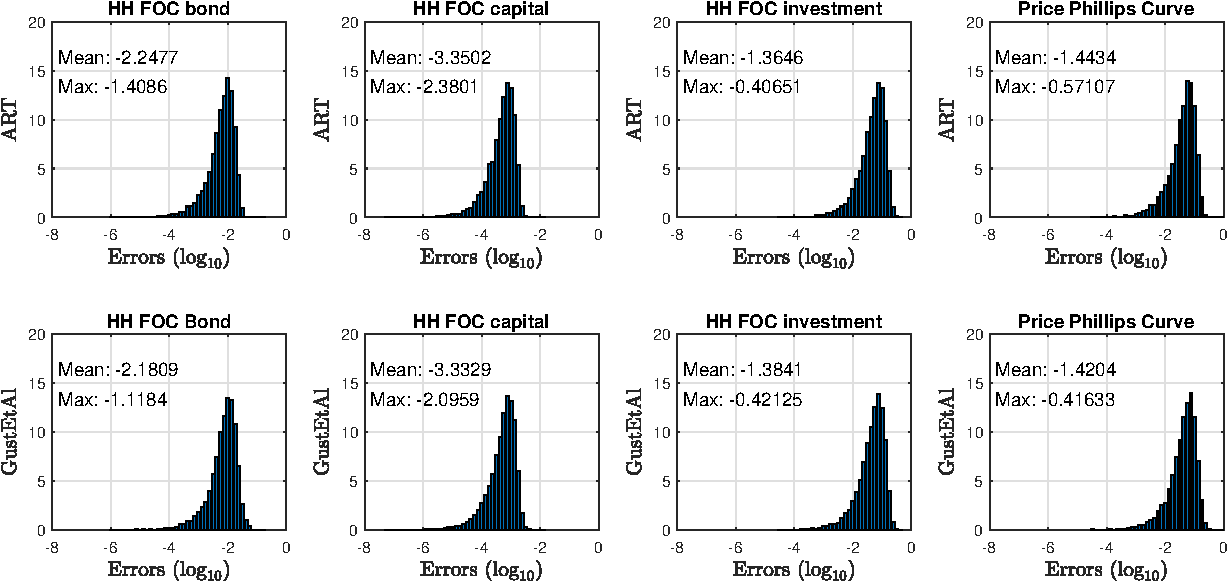
\includegraphics[width=16cm,scale=.8]{eeerrorsCAP.pdf}%{pfs3D_CAPITAL.pdf}
  \caption{Euler equation errors for model with capital}    
  \end{figure}

\subsection{Euler Equation Errors} \hyperlink{Figure 3}{Figure 3} shows the distribution of the absolute value of the Euler equation errors in base 10 logarithms for the household FOC bond, FOC capital, FOC investment, and price Phillips curve in the model with capital. We also report the mean and maximum error. %The corresponding results for the model without capital is reported in \hyperlink{Appendix C}{Appendix C}.

The Euler equation errors are comparable between solution algorithms. The household FOC bond and the price Phillips curve are slightly more negative thought the Euler equation errors are slightly more negative in general, and thus correspond to a smaller household error. The shapes of the errors are similar. %though the ART
%Euler equation errors are slightly more negative, and thus correspond to a smaller household error.
%The mean errors are similar, though the GHLS maximum errors are larger.


\begin{figure}[H]
\hypertarget{Figure 4}  
    \centering
\captionsetup{justification=centering}
    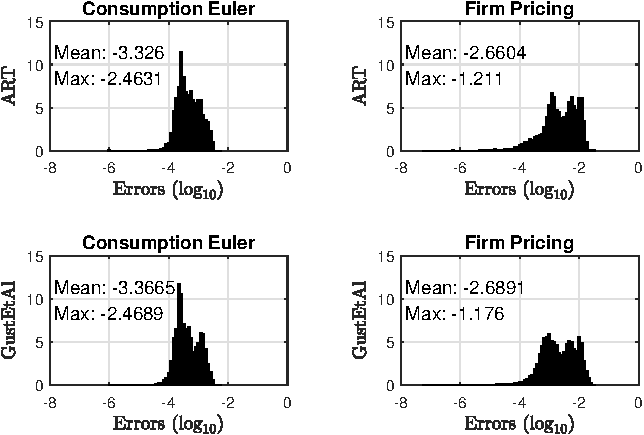
\includegraphics[scale=1]{eeerrors.pdf}
  \caption{Euler equation errors for model without capital}    
  \end{figure}

\hyperlink{Figure 4}{Figure 4} shows the distribution of the absolute value of the Euler equation errors in base 10
logarithms for the consumption Euler equation and the price Phillips curve. The mean and maximum Euler equations are comparable between algorithms, although GHLS has slightly smaller errors. Unlike the model with capital, GHLS performs better. 


\section[Section 5]{Conclusion \hypertarget{Section 5}{}} 

During the Great Recession, the U.S. Federal Reserve lowered policy rates to zero, creating a kink in its policy rule, and calling into question traditional solution methods. Recent work has explored solving fully nonlinear models to represent the ZLB, but not much work has compared the performance of different nonlinear solution methods. This paper analyzes the impact of regime-indexing the policy functions on a nonlinear solution algorithm. We use a method based on \hyperlink{Atkinson}{\color{black}{Atkinson et al.\ (2019)}} to motivate directly approximating the policy functions and a method based on  \hyperlink{Gust}{\color{black}{Gust et al.\ (2017)}} to motivate regime-indexing the policy functions. Although the regime-indexed policy functions were meant to be smoother and easier to compute, the GHLS method yielded more nonlinear policy functions and was slower than the ART method in our model with capital. The regime-indexed policy functions also yielded a solution that was less accurate in terms of Euler equation errors in the model with capital. 

Future work includes solving the GHLS solution method using Smolyak discretization methods with Chebyshev polynomials. We would expect this to speed up the solution algorithm, but it might lead to a less accurate solution. This paper shows that the policy functions conditional on the ZLB binding are quite nonlinear in the model with capital, which means low-order Chebyshev polynomials as in \hyperlink{Gust}{\color{black}{Gust et al.\ (2017)}} will have a difficult time approximating them. The ultimate question is whether the speed gain outweighs any loss in accuracy.

\appendix
  \section{Detrended Equilibrium System} \hypertarget{Appendix A}
  \noindent
  \textbf{Medium-Scale Model} The detrended system includes (\ref{eq:1}), (\ref{eq:6}), (\ref{eq:15}), (\ref{eq:16}) and 
\begin{gather}
\tilde{y}_t= (\tilde{k}_{t-1}/g_t)^\alpha n_t^{1-\alpha},\\
r^k_t = \alpha mc_t g_t \tilde{y}_t/\tilde{k}_{t-1},\\
\tilde{w}_t = (1-\alpha)mc_t\tilde{y}_t/n_t,\\
\tilde{y}^{gdp}_t = [1-\varphi(\pi_t^{gap} - 1)^2/2]\tilde{y}_t,\\
y^g_t = g_t\tilde{y}^{gdp}_t/(\bar{g}\tilde{y}^{gdp}_{t-1}),\\
\tilde{\lambda}_t = \tilde{c}_t\ - h\tilde{c}_{t-1}/g_t,\\
\label{eq:m1}
\tilde{w}_t = \chi n_t^\eta \tilde{\lambda}_t,\\
\tilde{c}_t + \tilde{x}_t = \tilde{y}^{gdp}_t,\\
x^g_t = g_t\tilde{x}_t/(\bar{g}\tilde{x}_{t-1}),\\
\tilde{k}_t = (1-\delta)(\tilde{k}_{t-1}/g_t) + \tilde{x}_t(1-\nu(x^g_t-1)^2/2),\\%%%
\label{eq:m2}
  1 = \beta E_t[(\tilde{\lambda}_t/\tilde{\lambda}_{t+1})(s_ti_t/(\bar{\pi}\pi_{t+1}^{gap}g_{t+1}))],\\
q_t = \beta E_t[(\tilde{\lambda}_t/\tilde{\lambda}_{t+1})(r^k_{t+1} + (1-\delta)q_{t+1})/g_{t+1}],\\
1 = q_t[1 - \nu(x^g_t-1)^2/2 - \nu(x^g_t-1)x^g_t] + \nu\beta\bar{g}E_t[q_{t+1}(\tilde{\lambda}_t/\tilde{\lambda}_{t+1})(x^g_{t+1})^2(x^g_{t+1}-1)/g_{t+1}],\\
\label{eq:m3}
  \varphi(\pi_t^{gap}-1){\pi}_t^{gap} = 1-\theta + \theta mc_t + \beta\varphi E_t[(\tilde{\lambda}_t/\tilde{\lambda}_{t+1}) (\pi_{t+1}^{gap}-1)\pi_{t+1}^{gap}(\tilde{y}_{t+1}/\tilde{y}_t)].
\end{gather}
The variables are $\tilde{c},\tilde{n},\tilde{x},\tilde{k},\tilde{y^{gdp}},\tilde{y},x^g,y^g,\tilde{w},r^k,\pi,i,i^n,q,mc,\tilde{\lambda},g,$ and $s$.\\

\noindent \textbf{Small-Scale Model} The detrended system includes (\ref{eq:1}), (\ref{eq:6}), (\ref{eq:15}), (\ref{eq:16}), (\ref{eq:m1}), (\ref{eq:m2}), (\ref{eq:m3}), and 
\begin{gather}
\tilde{\lambda}_t = \tilde{c}_t,\\ %%%
\tilde{c}_t = [1-\varphi(\pi_t^{gap} - 1)^2/2]\tilde{y}_t,\\ %%%
  \tilde{y}_t= n_t.  %%% 
\end{gather}
The variables are $\tilde{c},i^n,i,\tilde{\lambda},\tilde{w},\pi^{gap},\tilde{y},n,g,$ and $s$.\\ 

\section{Nonlinear Solution Method}\hypertarget{Appendix B}
The following discussion is based on \hyperlink{Atkinson}{\color{black}{Atkinson et al.\ (2019)}} and \hyperlink{RT}{\color{black}{Richter and Throckmorton (2014)}}. We express the detrended nonlinear system compactly as
\begin{gather*}
  E[f(\textbf{s}_{t+1},\textbf{s}_t,\varepsilon_{t+1})|\textbf{z}_t,\vartheta] = 0,
\end{gather*}
where $f$ is a vector-valued function, $\textbf{s}_t$ is a vector of variables, $\varepsilon_t \equiv [\varepsilon_{s,t}, \varepsilon_{g,t},\varepsilon_{i,t}]'$ is a vector of shocks, $\textbf{z}_t$ is a vector of states ($\textbf{z}_t \equiv [\tilde{c}_{-1}, i^n_{t-1},\tilde{k}_{t-1},\tilde{x}_{t-1},s_t,g_t,\varepsilon_{i,t}]'$ for the model with capital and $\textbf{z}_t \equiv [\tilde{c}_{t-1},i^n_{t-1},s_t,g_t,\varepsilon_{i,t}]'$ for the model without capital), and $\vartheta$ is a vector of parameters.

We use the Markov chain method in \hyperlink{Rouwenhorst}{\color{black}{Rouwenhorst (1995)}} to discretize the endogenous state variables, $s_t$, $g_t$, and $\varepsilon_{i,t}$ following ART. The bounds on $\tilde{c}_{t-1}, i^n_{t-1}, \tilde{k}_{t-1},$ and $\tilde{x}_{t-1}$ are set to $\pm 2.5\%$, $\pm 6\%$, $\pm 8\%$, and $\pm 15\%$, respectively, following \hyperlink{Atkinson}{\color{black}{Atkinson et al.\ (2019)}}. We discretize the states into 5 evenly-spaced points for the model with capital and 7 evenly-spaced points for the model without capital. The product of the points in each dimension, D, represents the total nodes in the state space ($D = 78125$ for the model with capital and $D = 2401$ for the model without capital). The realization of $\textbf{z}_t$ on node $d$ is denoted $\textbf{z}_t(d)$. The Rouwenhorst method provides integration nodes, $[s_{t+1}(m), g_{t+1}(m), \varepsilon_{i,t+1}(m)]$, with weights, $\phi(m)$, for $m \in \{1, \dots, M\}$.

The vector of policy functions is denoted $\textbf{pf}_t$ and the realization on node $d$ is denoted $\textbf{pf}_t(d)$ ($\textbf{pf}_t(d) \equiv [\tilde{\pi}^{gap}_t(\textbf{z}_t), n_t(\textbf{z}_t), q_t(\textbf{z}_t), mc_t(\textbf{z}_t)]$ for the model with capital and $\textbf{pf}_t(d) \equiv [\tilde{\pi}^{gap}_t(\textbf{z}_t), \tilde{c}_t(\textbf{z}_t)]$ for the model without capital. For the GHRT policy functions, any variables directly dependent on the interest rate ($n_t$ for the model with capital and $\tilde{c}_t$ for the model without capital) are the result of computing regime-indexed policy functions using (\ref{eq:18}) and (\ref{eq:19}). The policy functions are selected so that solving for other variables in the nonlinear system is straightforward. 

The following steps outline the global policy function iteration algorithm:

\begin{enumerate}
  \item Use Sims's (2002) \texttt{gensys} algorithm to solve the log-linear model without the ZLB constraint and obtain conjectures for the policy functions $\textbf{pf}_0$. (For GHLS, the initial guesses for $n_t^{normal}$ and $n_t^{ZLB}$ are set to the log-linear solution for $n_t$ from \texttt{gensys}).
  \item On each node $d \in \{1,\dots,D\}$:% use fixed point iteration to find $\textbf{pf}_t(d)$ to satisfy $E[f(\cdot)|\textbf{z}_t(d), \vartheta] \approx 0$. Guess $\textbf{pf}_j(d) = \textbf{pf}_{j-1}(d)$ Then: 
    \begin{enumerate}
    \item ART: Solve for all variables dated at time $t$, given $\textbf{pf}_t(d)$ and $\textbf{z}_t(d)$. \\
GHLS: Solve for $i_t$. If $i_t > 1$, solve for all time $t$ variables with $n_t^{normal}$. Otherwise, solve for all time $t$ variables with $n_t^{ZLB}$. 
    \item ART: Linearly interpolate the policy functions $\textbf{pf}_{j-1}$, at the updated state variables $\textbf{z}_{t+1}(m)$, to obtain $\textbf{pf}_{t+1}(m)$ on every integration node, $m \in \{1,\dots,M\}$.\\
GHLS: Linearly interpolate $n_t^{normal}$ and $n_t^{ZLB}$ in separate steps with the remainder of the policy functions in $\textbf{pf}_{j-1}$.
    \item ART: Given $\{\textbf{pf}_{t+1}(m)\}_{m=1}^M$, solve for the other elements of $\textbf{s}_{t+1}(m)$ and approximate the expectation operators
      \begin{gather*}
        E[f(\textbf{s}_{t+1},\textbf{s}_t(d),\varepsilon_{t+1})|\textbf{z}_t(d),\vartheta] \approx \sum_{m=1}^M \phi(m)f(\textbf{s}_{t+1}(m),\textbf{s}_t(d),\varepsilon_{t+1}(m)).
      \end{gather*}
GHLS: Solve for $\{i_t(m)\}_{m=1}^M$ using the interpolated policy functions and time $t$ variables. If the value of $\{i_t(m)\}_{m=1}^M$ on node $d$ is greater than 1, assign $\{n_t(m)\}_{m=1}^M$ on node $d$ to the corresponding value in $\{n_t^{normal}(m)\}_{m=1}^M$, otherwise assign $\{n_t(m)\}_{m=1}^M$ on node $d$ to the corresponding value in $\{n_t^{ZLB}(m)\}_{m=1}^M$. Solve for the other elements in $\textbf{s}_{t+1}$ and approximate the expectation operators.
      \item ART: Solve for $\textbf{pf}_t(d)$ from the expectation operators and $\textbf{s}_{t+1}(m)$. Set $\textbf{pf}_j(d) = \textbf{pf}_t(d)$.\\
GHLS: Using the expectation operators, solve for the $n_t(d)$ policy in the style of (\ref{eq:20}) and the $n_t^{ZLB}$ policy in the style of (\ref{eq:21}). Solve for the rest of the policy functions in $\textbf{pf}_t(d)$.  
    \end{enumerate}
       \item Repeat step 2 until $\text{maxdist}_j < 10^{-6}$, where $\text{maxdist}_j \equiv \text{max}\{|\textbf{pf}_j - \textbf{pf}_{j-1}|\}$. When that criterion is satisfied, the algorithm has converged to an approximate nonlinear solution.
\end{enumerate}

%\section{Results for model without capital} \hypertarget{Appendix C}
\section*{References}

\setlength\parindent{0pt}

\hypertarget{Aruoba} \hangindent=0.5cm \textsc{Aruoba, S., P. Cuba-Borda, and F. Schorfheide (2018):}  “Macroeconomic Dynamics
Near the ZLB: A Tale of Two Countries,”  \textit{The Review of Economic Studies}, 85, 87-118.

\hypertarget{Atkinson}\hangindent=0.5cm \textsc{Atkinson, T., A. W. Richter, N. A. Throckmorton (2019):} “The Accuracy of Linear and Nonlinear Estimation in the
Presence of the Zero Lower Bound,” FRB Dallas Working Paper 1705, revised February 2019. 
 
\hypertarget{Christiano}\hangindent=0.5cm \textsc{Christiano, L. J., and J. D. M. Fisher (2000): } “Algorithms for Solving Dynamic Models with Occasionally Binding
Constraints,” \textit{Journal of Economic Dynamics and Control}, 24 (8), 1179-1232.

\hypertarget{Fernald}\hangindent=0.5cm \textsc{Fernald, J. G. (2012):}   “A Quarterly, Utilization-Adjusted Series on Total Factor Productivity,” Federal Reserve Bank of San Francisco Working Paper 2012-19.

\hypertarget{Fernandez}\hangindent=0.5cm \textsc{Ferna\'ndez-Villaverde, J., G. Gordon, P. Guerro\'n-Quintana, and J. F.
Rubio-Rami\'rez (2015):}  “Nonlinear Adventures at the Zero Lower Bound,” \textit{Journal of
Economic Dynamics and Control}, 57, 182-204.

\hypertarget{Guerrieri}\hangindent=0.5cm\textsc{Guerrieri, L. and M. Iacoviello (2015):} “OccBin: A toolkit for solving dynamic models with occasionally binding
constraints easily,”  \textit{Journal of Monetary Economics}, 70, 22-38.

\hypertarget{Gust}\hangindent=0.5cm\textsc{Gust, C., E. Herbst, D. Lo\'pez-Salido, and M. E. Smith (2017):} “The Empirical Implications of the Interest-Rate
Lower Bound,”  \textit{American Economic Review}, 107, 1971-2006.

\hypertarget{Judd1} \hangindent=0.5cm \textsc{Judd, K. L., Maliar, L. and Maliar, S. (2010)}   “A Cluster-Grid Projection Method: Solving Problems with High Dimensionality” \textit{Computational Economics}, NBER Working Paper, 15965.

\hypertarget{Judd2}\hangindent=0.5cm\textsc{Judd, K. L., L. Maliar, S. Maliar, and R. Valero (2014):}  “Smolyak Method for Solving Dynamic Economic Models:
Lagrange Interpolation, Anisotropic Grid and Adaptive Domain,”  \textit{Journal of Economic Dynamics and Control}, 44, 92-123.

\hypertarget{Den}\hangindent=0.5cm\textsc{Den Haan, W. J. and Marcet A. (1994):}  “Accuracy in Simulations,"  \textit{Review of Economic Studies}, 61(1), 3-17.

\hypertarget{Kopecky}\hangindent=0.5cm\textsc{Kopecky, K. and R. Suen (2010):} “Finite State Markov-chain Approximations to Highly
Persistent Processes,” \textit{Review of Economic Dynamics}, 13, 701-714.

\hypertarget{Peterman}\hangindent=0.5cm \textsc{Peterman, W. B. (2016):}  “Reconciling Micro and Macro Estimates of the Frisch Labor Supply
Elasticity,” \textit{Economic Inquiry}, 54, 100-120.

\hypertarget{Plante}\hangindent=0.5cm\textsc{Plante, M., A. W. Richter, and N. A. Throckmorton (2018):}  “The Zero Lower Bound and Endogenous Uncertainty,” \textit{Economic Journal}, forthcoming.
\hypertarget{RT}\hangindent=0.5cm \textsc{Richter, A. W. and N. A. Throckmorton (2016):}  “Is Rotemberg Pricing Justified by Macro Data?” \textit{Economics Letters}, 149, 44-48.

\hypertarget{RWT}\hangindent=0.5cm\textsc{Richter, A. W., N. A. Throckmorton, and T. B. Walker (2014):}  “Accuracy, Speed and Robustness of Policy Function Iteration,” \textit{Computational Economics}, 44, 445-476.

\hypertarget{Rotemberg}\hangindent=0.5cm \textsc{Rotemberg, J. J. (1982):} “Sticky Prices in the United States,” \textit{Journal of Political Economy}, 90, 1187-1211.

\hypertarget{Rouwenhorst}\hangindent=0.5cm \textsc{Rouwenhorst, K. G. (1995):}  “Asset Pricing Implications of Equilibrium Business Cycle
Models,” in \textit{Frontiers of Business Cycle Research}, ed. by T. F. Cooley, Princeton, NJ: Princeton
University Press, 294-330.

\hypertarget{Sims}\hangindent=0.5cm \textsc{Sims, C. A. (2002):}  “Solving Linear Rational Expectations Models,” \textit{Computational Economics}, 20, 1-20.

\hypertarget{Smolyak}\hangindent=0.5cm\textsc{Smolyak, S. (1963):} “Quadrature and interpolation formulas for tensor products of certain classes of functions,” \textit{Dokl. Akad. Nauk}, 148, 1042-1045. 

%\hangindent=0.5cm\textsc{Aruoba, S. B., J. Fernandez-Villaverde, J. F. Rubio-Ramirez (2006):} “Comparing solution methods for dynamic equilibrium economies,” \textit{Journal of Economic Dynamics and Control}, 30, 2477-2508.
%\hangindent=0.5cm








 
\end{document}

